% 村松先生とのミーティング（2026年11月2日（月）17:00 JST / 9:00 CET）用
% NEM（Neighbored Element Method）の基礎と、10月6日に届いた資料
%
% ビルド: lualatex slides_1102_nem_ja.tex   （2回）
% CONSTRAINT: 20 ページ以内。エラー 0、Overfull 0 を確認してから渡す。
%
% Felix Klempt の実装・理論の章・入力ファイルは非公開（CLAUDE.md）。このスライドには
% 中身を書かない。書いてよいのは「受け取った」「照合している」ことと、公開済みの論文の内容だけ。
% 彼の資料に基づく内容を足すときは、先に本人の了解を取る。
\documentclass[aspectratio=169,11pt]{beamer}
\usepackage{luatexja}
\usetheme{Madrid}
\usecolortheme{seahorse}
\usepackage{booktabs}
\usepackage{amsmath,amssymb}
\usepackage{bm}
\usepackage{xcolor}
\usepackage{graphicx}
\usepackage{tikz}
\usetikzlibrary{arrows.meta,positioning}

\definecolor{c3}{RGB}{30,80,160}
\setbeamercolor{frametitle}{bg=c3, fg=white}
\setbeamertemplate{navigation symbols}{}
\tikzset{box/.style={draw,rounded corners,align=center,font=\footnotesize,minimum height=1.0cm,text width=#1},
  box/.default=3.0cm,
  fem/.style={box,fill=gray!15},
  nem/.style={box,fill=c3!15,draw=c3},
  arr/.style={-{Latex[length=2mm]},thick}}

\title{Neighbored Element Method（NEM）の基礎}
\subtitle{相方の ANSYS 要素の場の解き方と，慶應での数値面の研究}
\author[西岡佳祐]{西岡佳祐}
\institute[IKM, LUH / 慶應]{%
\small ライプニッツ大学ハノーファー 連続体力学研究所（IKM）\\
\small 慶應義塾大学}
\date{2026年11月2日}

\begin{document}
\maketitle

% --------------------------------------------------------
\begin{frame}{お話しする順番}
\begin{enumerate}
  \item 10月6日に届いた資料
  \item NEM の考え方：Taylor 展開と重み付き最小二乗
  \item 陽解法の時間刻みと，私の計算条件
  \item 精度と計算コスト（Rudolf et al.\ 2025）
  \item ANSYS（NEM）と Abaqus（通常の有限要素）の違い
  \item 慶應で続ける数値面の研究と，ご相談したいこと
\end{enumerate}
\end{frame}

% --------------------------------------------------------
\begin{frame}{1. 10月6日に届いた資料}
\small
\begin{tabular}{p{0.32\linewidth}p{0.19\linewidth}p{0.37\linewidth}}
\toprule
資料 & 送り主 & 扱い \\
\midrule
NEM の論文 7 本 & F.\ Klempt（IKM） & 公開。4 本はオープンアクセスでリポジトリに収録，3 本は引用のみ \\
相方の要素の最新版（2 菌種，2 栄養） & F.\ Klempt & \textbf{非公開}。照合中 \\
2 菌種モデルの理論（博士論文の章） & F.\ Klempt & \textbf{非公開}。本人の了解なしに共有しない \\
ANSYS Workbench の入力 & F.\ Klempt & \textbf{非公開}。使った値を照合中 \\
\bottomrule
\end{tabular}

\vspace{8pt}
\begin{itemize}
  \item 非公開の資料は，私の手元のパソコンの中だけに置いています。このスライドには中身を書いていません。
  \item Felix から，2 菌種モデルで一緒に論文を書く提案がありました（Soleimani 先生，Junker 先生の同意が前提）。
  \item 今日は，公開されている NEM の論文の内容をお話しします。
\end{itemize}
\end{frame}

% --------------------------------------------------------
\begin{frame}{2. NEM が解く問題}
成長の場 $\phi$（Klempt et al.\ 2024，Eq.\ 34）は拡散の項を持つ放物型の方程式です。
\[
  \dot\phi=\beta\,\nabla^2\phi+(\text{局所の成長})+(\text{前線の項}),\qquad
  \mathbf n\cdot\nabla\phi=0\ \text{（境界）}
\]
\vspace{-4pt}
\begin{columns}[T]
\begin{column}{0.48\textwidth}
\colorbox{gray!12}{\parbox{0.95\linewidth}{\small
\textbf{通常の有限要素（Abaqus で使用）}\\[2pt]
$\phi$ を節点の自由度にする。変位と同じ連立方程式に入るので，式の数が増える。陰解法にできる。}}
\end{column}
\begin{column}{0.48\textwidth}
\colorbox{c3!12}{\parbox{0.95\linewidth}{\small
\textbf{NEM（相方の ANSYS 要素）}\\[2pt]
$\phi$ を積分点の内部変数にする。$\nabla^2\phi$ と $\nabla\phi$ は近くの点の値から近似する。
連立方程式は変位だけで，$\phi$ は陽解法で進める。}}
\end{column}
\end{columns}
\vspace{8pt}
{\small もとはトポロジー最適化（密度）と勾配型の損傷モデル（損傷変数）のために，Junker 先生のグループで作られた方法です。}
\end{frame}

% --------------------------------------------------------
\begin{frame}{NEM の1ステップ}
\centering
\begin{tikzpicture}[node distance=0.5cm and 0.9cm]
\node[nem] (d) {係数行列 $\mathbf D$\\ メッシュごとに1回};
\node[fem,right=of d] (u) {変位を解く（FEM）\\ 前のステップの $\phi$ を使う};
\node[fem,right=of u] (s) {応力 $\boldsymbol\sigma$};
\node[nem,below=1.0cm of s] (l) {$\nabla^2\phi\approx\mathbf D\,\mathbf b$\\ 近傍の値の差 $\mathbf b$};
\node[nem,left=of l] (p) {$\phi$ を陽解法で更新};
\node[box,left=of p,draw=none] (n) {次のステップへ};
\draw[arr] (d)--(u); \draw[arr] (u)--(s); \draw[arr] (s)--(l); \draw[arr] (l)--(p); \draw[arr] (p)--(n);
\draw[arr,dashed] (d.south) |- (l.west);
\end{tikzpicture}

\vspace{10pt}
\begin{itemize}\small
  \item 力学と場は交互（staggered）に解きます。場の更新は連立方程式を解かないので，追加の計算はわずかです。
  \item $\mathbf D$ は点の位置だけで決まります。初期条件を変えても作り直す必要はありません。
\end{itemize}
\end{frame}

% --------------------------------------------------------
\begin{frame}{3. 2 次の Taylor 展開と重み付き最小二乗}
\small
点 $\mathbf x_0$ のまわりで，近くの点 $\mathbf x_i=\mathbf x_0+\Delta\mathbf x_i$（$i=1,\dots,n$）に Taylor 展開を当てはめます（Blaszczyk et al.\ 2022；Rudolf et al.\ 2025，Eq.\ 4--13）。
\[
  \phi_i-\phi_0\approx
  \tfrac12\Delta x_i^2\,\phi_{,xx}+\tfrac12\Delta y_i^2\,\phi_{,yy}+\tfrac12\Delta z_i^2\,\phi_{,zz}
  +\Delta x_i\Delta y_i\,\phi_{,xy}+\dots+\Delta x_i\,\phi_{,x}+\Delta y_i\,\phi_{,y}+\Delta z_i\,\phi_{,z}
\]
未知数は 9 個の微分 $\mathbf m$ です。$n>9$ 点を使い，$\mathbf A\mathbf m\approx\mathbf b$ を重み付き最小二乗で解きます。
\[
  \min_{\mathbf m}\,(\mathbf A\mathbf m-\mathbf b)^{\mathsf T}\mathbf W(\mathbf A\mathbf m-\mathbf b)
  \quad\Rightarrow\quad
  \mathbf m=\underbrace{(\mathbf A^{\mathsf T}\mathbf W\mathbf A)^{-1}\mathbf A^{\mathsf T}\mathbf W}_{\mathbf D}\,\mathbf b,
  \qquad
  W_{ii}=\exp\!\Big(-\tfrac12\big(\tfrac{4d_i}{\beta^\star}\big)^2\Big)
\]
\begin{itemize}
  \item $\nabla^2\phi\approx m_1+m_2+m_3=\sum_j L_j\,(\phi_j-\phi_0)$：近傍の値の重み付きの和になります。
  \item 逆行列は $9\times9$ だけで，近傍の数によりません。$\beta^\star$ は重みの幅です（Klempt の $\beta$ とは別の量）。
  \item 境界では $\mathbf n\cdot\nabla\phi=0$ の行を 1 行足します。
  \item 相方の要素：$\phi$ は積分点（要素あたり 8 点）にあり，近傍は約 30 点です。
\end{itemize}
\end{frame}

% --------------------------------------------------------
\begin{frame}{この近似を自分で確かめた例}
\centering
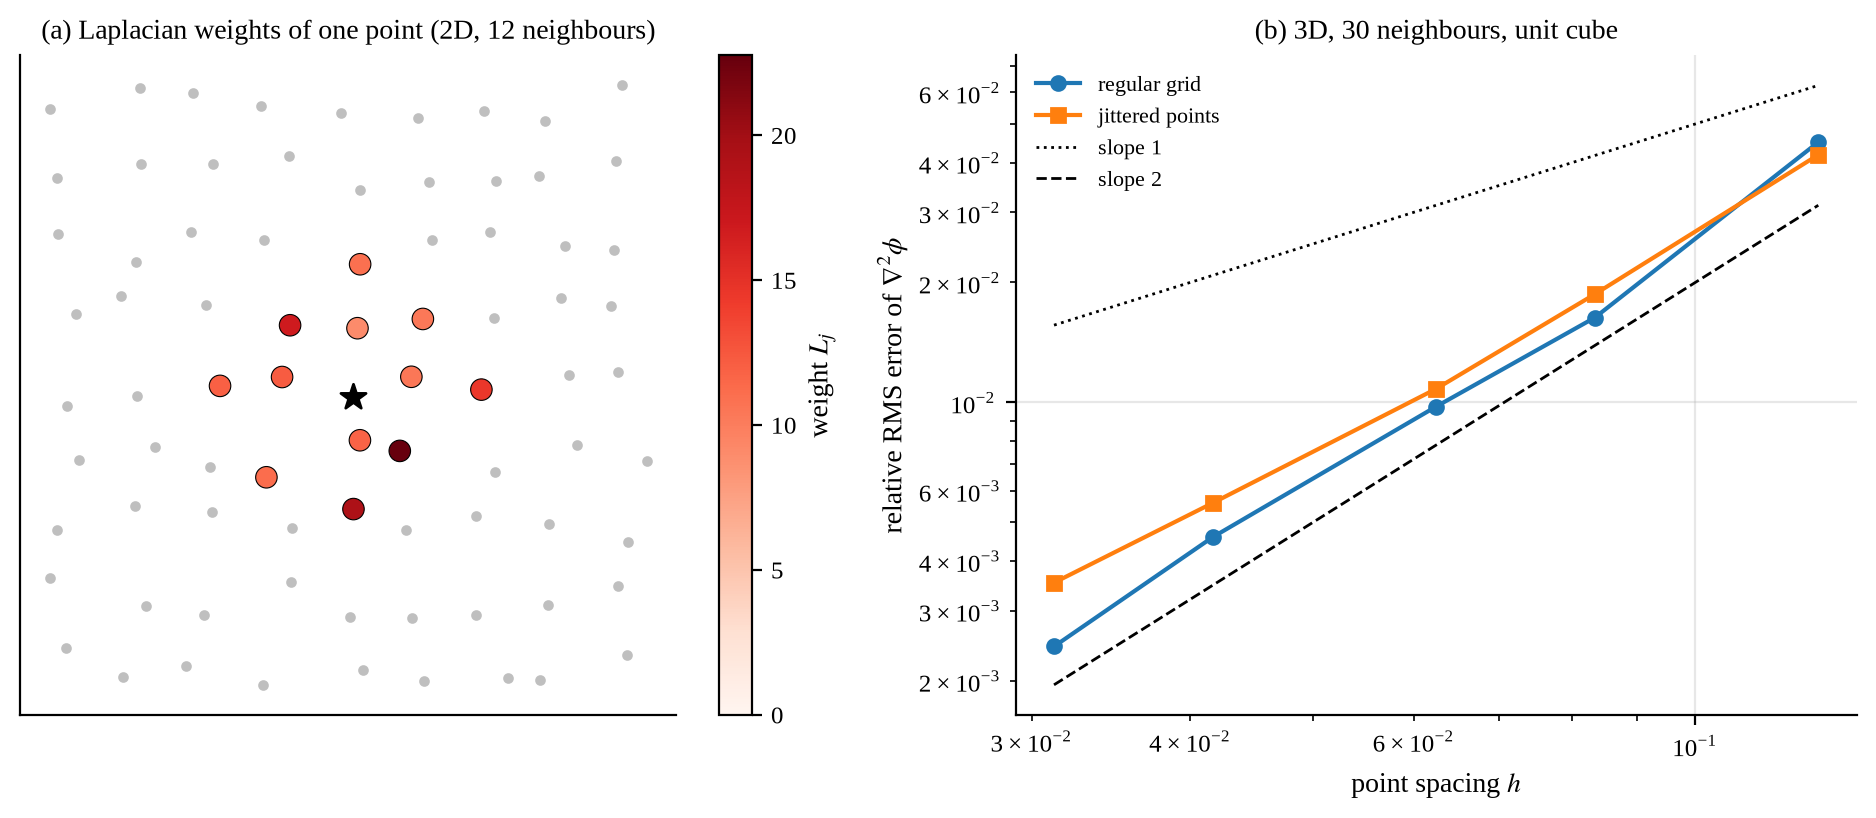
\includegraphics[width=0.86\linewidth]{assets/fig_nem_demo.png}

\small
(a) 不規則な点での 1 点の重み $L_j$（2 次元）。(b) 3 次元の $\phi=\sin\pi x\,\sin\pi y\,\sin\pi z$ で，
$\nabla^2\phi$ の誤差は点の間隔 $h$ にほぼ 2 次で減ります。不規則な点では少し遅くなります。\\
{\footnotesize 説明用の Python の実装で，相方の要素のコードではありません。}
\end{frame}

% --------------------------------------------------------
\begin{frame}{4. 陽解法の時間刻みと，私の計算条件}
陽解法なので，時間刻みに上限があります（Rudolf et al.\ 2025，Eq.\ 3）。
\[
  \frac{h^2}{2\,\Delta t}\ \ge\ \beta
\]
\begin{center}
\begin{tabular}{lccc}
\toprule
メッシュ（2 mm の立方体） & $8^3$ & $16^3$ & $24^3$ \\
\midrule
要素の大きさ $h$ [mm] & 0.25 & 0.125 & 0.083 \\
$h^2/(2\Delta t)$，$\Delta t=0.025$ [mm$^2/T^*$] & 1.25 & 0.31 & 0.14 \\
\bottomrule
\end{tabular}
\end{center}
\begin{itemize}
  \item 私の $\beta=0.02$\,mm$^2/T^*$ は，どのメッシュでも条件を満たします（$\beta$ は Klempt 2024 Table 2 を換算した仮定）。
  \item 相方の入力例の $\beta=10^{-4}$ も安定ですが，拡散の長さ（約 0.01 mm）が要素より小さく，シードの応力がメッシュで収束しません。これは NEM の誤差ではなく，解像度の問題です。
  \item 前線の項は移流のような項なので，別の上限が加わります。細かいメッシュでは時間刻みも小さくします。
\end{itemize}
\end{frame}

% --------------------------------------------------------
\begin{frame}{5. 精度と計算コスト（Rudolf et al.\ 2025）}
\small
ANSYS の熱伝導要素（陰解法の一体解法）と，同じメッシュで比べています。
\begin{columns}[T]
\begin{column}{0.5\textwidth}
\textbf{精度}（4 分の 1 トーラス，熱と力学）
\begin{itemize}
  \item 差の平均は 1\,\% 未満
  \item メッシュを細かくすると 1 次で収束
  \item 四面体は六面体より誤差が大きい（近傍点の配置の偏り）
  \item 重みの幅 $\beta^\star$ の影響は 0.3\,\% 以下
\end{itemize}
\end{column}
\begin{column}{0.48\textwidth}
\textbf{コスト}（立方体，約 62 万節点）
\begin{itemize}
  \item 直接法同士で 5〜10 倍速い
  \item 反復法にすると 155 倍速く，メモリは 1/77
  \item 利点の一部は交互解法から来る，と著者自身が書いています
\end{itemize}
\end{column}
\end{columns}
\vspace{8pt}
\colorbox{c3!12}{\parbox{0.97\linewidth}{\small
論文の「今後の課題」：市販コードの交互解法との比較。$\to$ 慶應での Abaqus との比較が，そのまま当たります。}}
\end{frame}

% --------------------------------------------------------
\begin{frame}{6. ANSYS（NEM）と Abaqus（通常の有限要素）}
\small
\begin{tabular}{p{0.22\linewidth}p{0.32\linewidth}p{0.32\linewidth}}
\toprule
 & 相方の ANSYS 要素 & 私の Abaqus 版（慶應で継続） \\
\midrule
$\phi$ の置き場所 & 積分点（内部変数） & 節点（温度の自由度，UMATHT） \\
$\nabla^2\phi$ & Taylor 展開＋重み付き最小二乗 & Galerkin（形状関数） \\
時間積分 & 陽解法 & 陰解法 \\
時間刻み & 安定条件で上限あり & 精度で決める \\
栄養 $c$ & 同じ近似で準定常の連立方程式 & 別の要素（UEL）で準定常 \\
連立方程式の大きさ & 変位だけ & 変位＋$\phi$ \\
\bottomrule
\end{tabular}

\vspace{8pt}
\begin{itemize}
  \item 近似の仕方が違うので，二つが最後の桁まで一致することは期待しません。メッシュを細かくしたときに同じ値へ近づくかで比べます。
  \item Abaqus 版は $48^3$ までメッシュ収束を確かめています。
\end{itemize}
\end{frame}

% --------------------------------------------------------
\begin{frame}{NEM の論文の流れ}
\small
\begin{tabular}{p{0.34\linewidth}p{0.58\linewidth}}
\toprule
論文 & 加えたこと \\
\midrule
Jantos, Hackl, Junker (2019) & トポロジー最適化の密度に，近傍の Taylor 展開と陽解法 \\
Junker et al.\ (2019) & 勾配型の脆性損傷へ。名前が NEM になる \\
Vogel, Junker (2020) & 同じ損傷モデルを適応的な有限要素で解いた参照解 \\
Blaszczyk, Jantos, Junker (2022) & 重み付き最小二乗で，任意の点の配置と Neumann 境界に対応 \\
Junker, Riesselmann, Balzani (2022) & 有限ひずみ，要素の除去 \\
Rudolf et al.\ (2025) & 精度とコストを ANSYS と比較（著者に Klempt，Soleimani） \\
von Zabiensky, Jantos, Junker (2026) & 接触の第 3 媒体の正則化に応用 \\
\bottomrule
\end{tabular}

\vspace{8pt}
{\small 詳しい人：Tobias Rudolf，Ilayda Kök，May von Zabiensky（IKM）}
\end{frame}

% --------------------------------------------------------
\begin{frame}{修論の連成と，慶應で足す 2 本の矢印}
\centering
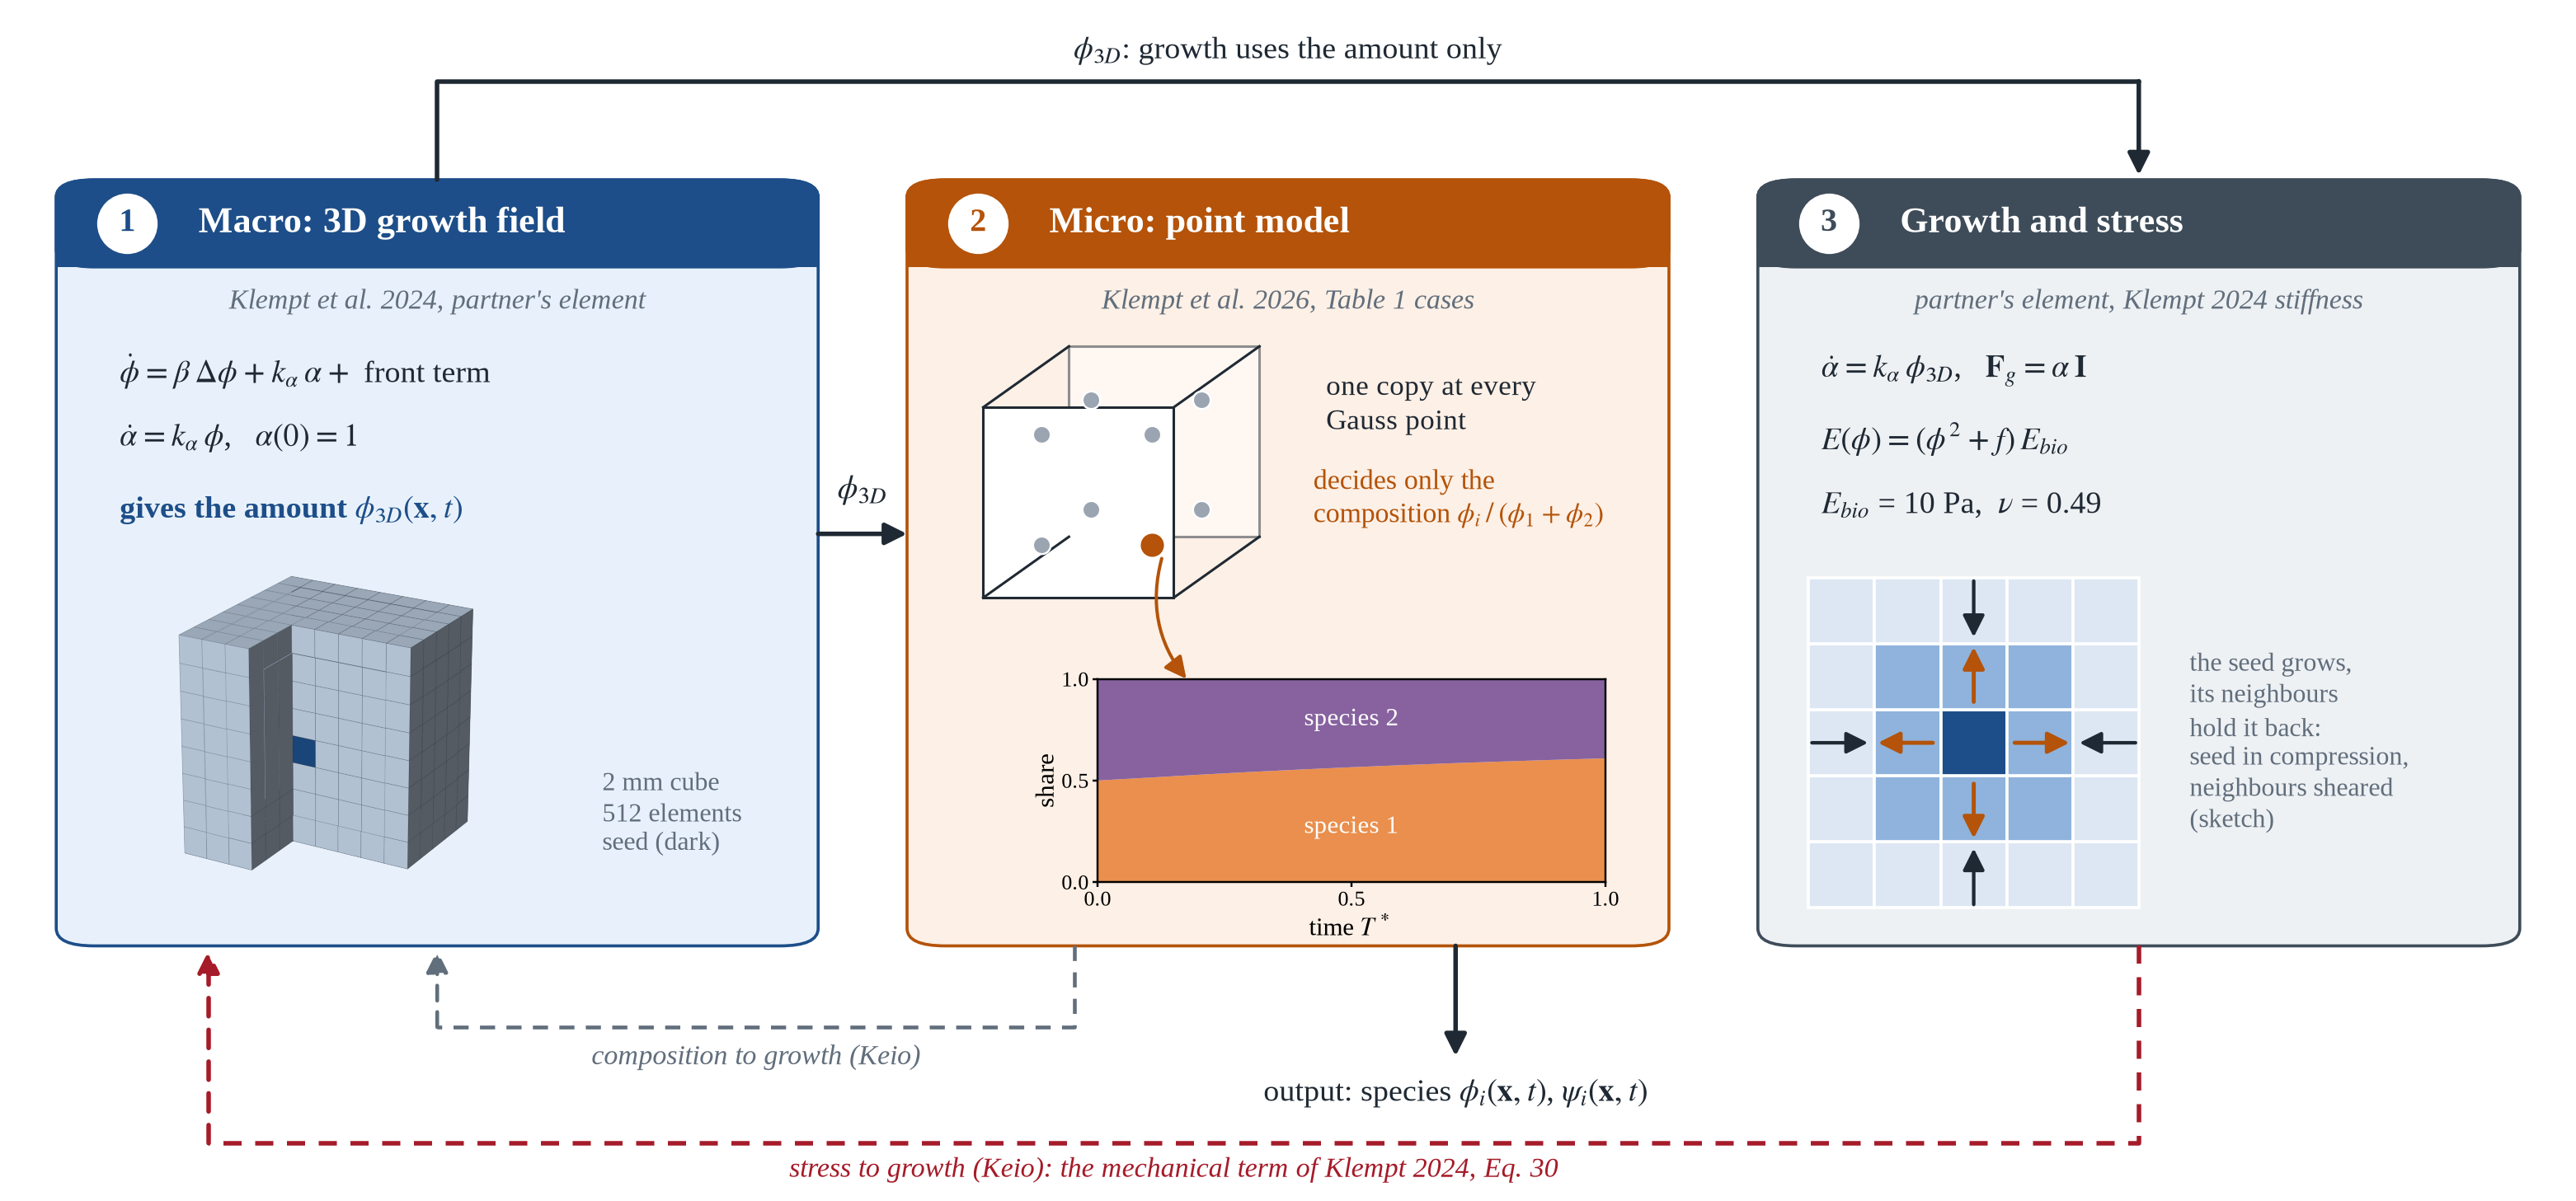
\includegraphics[width=0.90\linewidth]{assets/fig_coupling_schematic_keio.png}

\small
修論は一方向：場が量 $\phi$ を決め，点モデルが組成を決め，成長と応力は量だけを使う。\\
慶應で足すのは赤と灰色の点線：応力から成長へ（本体），組成から成長へ。
\end{frame}

% --------------------------------------------------------
\begin{frame}{7. 慶應で続ける数値面の研究（案）}
\begin{enumerate}\small
  \item \textbf{NEM と Galerkin の比較。} 同じ成長の問題（Klempt 2024 の例題）を，ANSYS の NEM と Abaqus の通常の有限要素で解き，
        メッシュ収束，時間刻み，計算時間を比べる。Rudolf et al.\ が残した課題に当たる。
  \item \textbf{シード表面の $\alpha$ の段差。} 段差の大きさと $\beta$，メッシュの関係（$8^3$/$16^3$/$24^3$ の結果あり）。
  \item \textbf{点モデルを置く場所。} 組成の点モデルを積分点に置くか，節点に置くか。
  \item \textbf{応力から成長へ（本体）。} 応力が場に戻ると交互解法で足りるかが問題になる。NEM は交互解法が前提なので，ここで違いが出る。
\end{enumerate}
\vspace{4pt}
{\small 1〜3 は修論の続きとしてすぐ始められます。4 は Felix の 2 菌種モデルとの共同研究とも重なります。}
\end{frame}

% --------------------------------------------------------
\begin{frame}{ご相談したいこと}
\begin{enumerate}
  \item 数値面（NEM と Galerkin の比較）を短い論文 1 本にする方向でよいか
  \item 応力から成長への成長則：研究室で扱っている成長・リモデリングのモデルで，使えるものはあるか
  \item Felix との共同研究（2 菌種モデル）と，慶應での研究の分け方
  \item 慶應の計算環境（Abaqus のライセンス，並列計算）
\end{enumerate}
\end{frame}

% --------------------------------------------------------
\begin{frame}{参考文献}
\scriptsize
\begin{itemize}
  \item F.\ Klempt, M.\ Soleimani, P.\ Wriggers, P.\ Junker: A Hamilton principle-based model for diffusion-driven biofilm growth. Biomech.\ Model.\ Mechanobiol.\ 23 (2024) 2091--2113.
  \item T.\ Rudolf, F.\ Klempt, H.\,I.\ Kök, M.\ Soleimani, D.\,R.\ Jantos, P.\ Junker: Computational efficiency and accuracy of the Neighbored Element Method. Finite Elem.\ Anal.\ Des.\ 249 (2025) 104353.
  \item M.\ Blaszczyk, D.\,R.\ Jantos, P.\ Junker: Application of Taylor series combined with the weighted least square method to thermodynamic topology optimization. Comput.\ Methods Appl.\ Mech.\ Eng.\ 393 (2022) 114698.
  \item D.\,R.\ Jantos, K.\ Hackl, P.\ Junker: An accurate and fast regularization approach to thermodynamic topology optimization. Int.\ J.\ Numer.\ Methods Eng.\ 117 (2019) 991--1017.
  \item P.\ Junker, S.\ Schwarz, D.\,R.\ Jantos, K.\ Hackl: A fast and robust numerical treatment of a gradient-enhanced model for brittle damage. Int.\ J.\ Multiscale Comput.\ Eng.\ 17 (2019).
  \item A.\ Vogel, P.\ Junker: Adaptive and highly accurate numerical treatment for a gradient-enhanced brittle damage model. Int.\ J.\ Numer.\ Methods Eng.\ 121 (2020) 3108--3131.
  \item E.\,K.\ Chu, O.\ Kilic, H.\ Cho, A.\ Groisman, A.\ Levchenko: Self-induced mechanical stress can trigger biofilm formation in uropathogenic \emph{Escherichia coli}. Nat.\ Commun.\ 9 (2018) 4087.
  \item P.\ Junker, J.\ Riesselmann, D.\ Balzani: Efficient and robust numerical treatment of a gradient-enhanced damage model at large deformations. Int.\ J.\ Numer.\ Methods Eng.\ 123 (2022) 774--793.
  \item M.\ von Zabiensky, D.\,R.\ Jantos, P.\ Junker: A fast and robust third medium contact approach using the neighbored element method. Finite Elem.\ Anal.\ Des.\ 255 (2026) 104489.
\end{itemize}
\end{frame}

% --------------------------------------------------------
\appendix
\begin{frame}{付録：記号}
\small
\begin{tabular}{lp{0.72\linewidth}}
\toprule
記号 & 意味 \\
\midrule
$\phi$ & バイオフィルムの体積分率（成長の場，Klempt 2024） \\
$c$ & 栄養の濃度 \\
$\alpha$ & 局所の成長，$\mathbf F_g=\alpha\mathbf I$，$\alpha(0)=1$ \\
$\beta$ & $\phi$ の拡散係数（Eq.\ 34）。この研究では 0.02 mm$^2/T^*$（仮定） \\
$\beta^\star$ & NEM の重みの幅（$\beta$ とは別の数値パラメータ） \\
$h$，$\Delta t$ & 要素の大きさ，時間刻み \\
$\mathbf A,\ \mathbf b,\ \mathbf m$ & Taylor 展開の係数行列，近傍との値の差，9 個の微分 \\
$\mathbf W,\ \mathbf D$ & 重みの対角行列，$\mathbf m=\mathbf D\mathbf b$ となる係数行列 \\
$L_j$ & 点 $j$ の Laplacian の重み，$\nabla^2\phi\approx\sum_j L_j(\phi_j-\phi_0)$ \\
$T^*$ & 無次元の時間（Klempt 2024） \\
$p$，$p_h$，$P_h$ & 圧力（圧縮が正），恒常圧，その無次元の値（$p_h=P_h E k_\alpha T^*$） \\
$d,\ g,\ r,\ k$ & 栄養の拡散，消費（$g\phi c$），前線の速さ，半飽和定数（Eq.\ 34，35） \\
$w$ & 前線の項のうち全面で成長する割合（この研究の仮定） \\
$E,\ \nu,\ f$ & バイオフィルムのヤング率，ポアソン比，空所の剛性の下限 \\
\bottomrule
\end{tabular}
\end{frame}

% --------------------------------------------------------
\begin{frame}{付録（予備）：応力から成長へ，恒常圧の成長則}
\small
Klempt 2024 の Eq.\ 30 の力学の項 $\phi\mu(\mathbf I:\tilde{\mathbf C}_e-3)$ を $\phi$ の式に戻すと，Table 2 の値ではシードが消える（10月に確認）。
そこで成長の式の側に帰還を入れた：
\[
\dot\alpha = k_\alpha\,\phi\,\max\!\left(0,\ 1-\frac{p}{p_h}\right),\qquad p=-\tfrac13\operatorname{tr}\boldsymbol\sigma\ \ (\text{圧縮が正})
\]
\begin{itemize}
  \item 閉じ込められたコロニーは圧力が約 10 kPa で成長を止める（Chu et al.\ 2018）。
  \item $p_h$ は 2 通り（仮定）：$p_h=P_h\,E\,k_\alpha T^*$，または局所の剛性に比例 $p_h=P_h\,E(\phi^2+f)\,k_\alpha T^*$。
  \item 形：インプラントのカラー部（半径 2.05 mm）と歯冠（半径が上へ 1 mm 広がる），厚さ 0.25 mm，高さ 2 mm の層。
        内側の面は剛体に接着。値はこの研究で決めたもので，論文の値ではない。
  \item 軸対称の Python 試作（$8\times64$ 要素），$E=10$ Pa，$\nu=0.49$，$\beta=0.02$ mm$^2/T^*$，$k_\alpha=10^{-3}$。
\end{itemize}
\end{frame}

% --------------------------------------------------------
\begin{frame}{付録（予備）：インプラントと歯，歯頸線に応力が集まる}
\centering
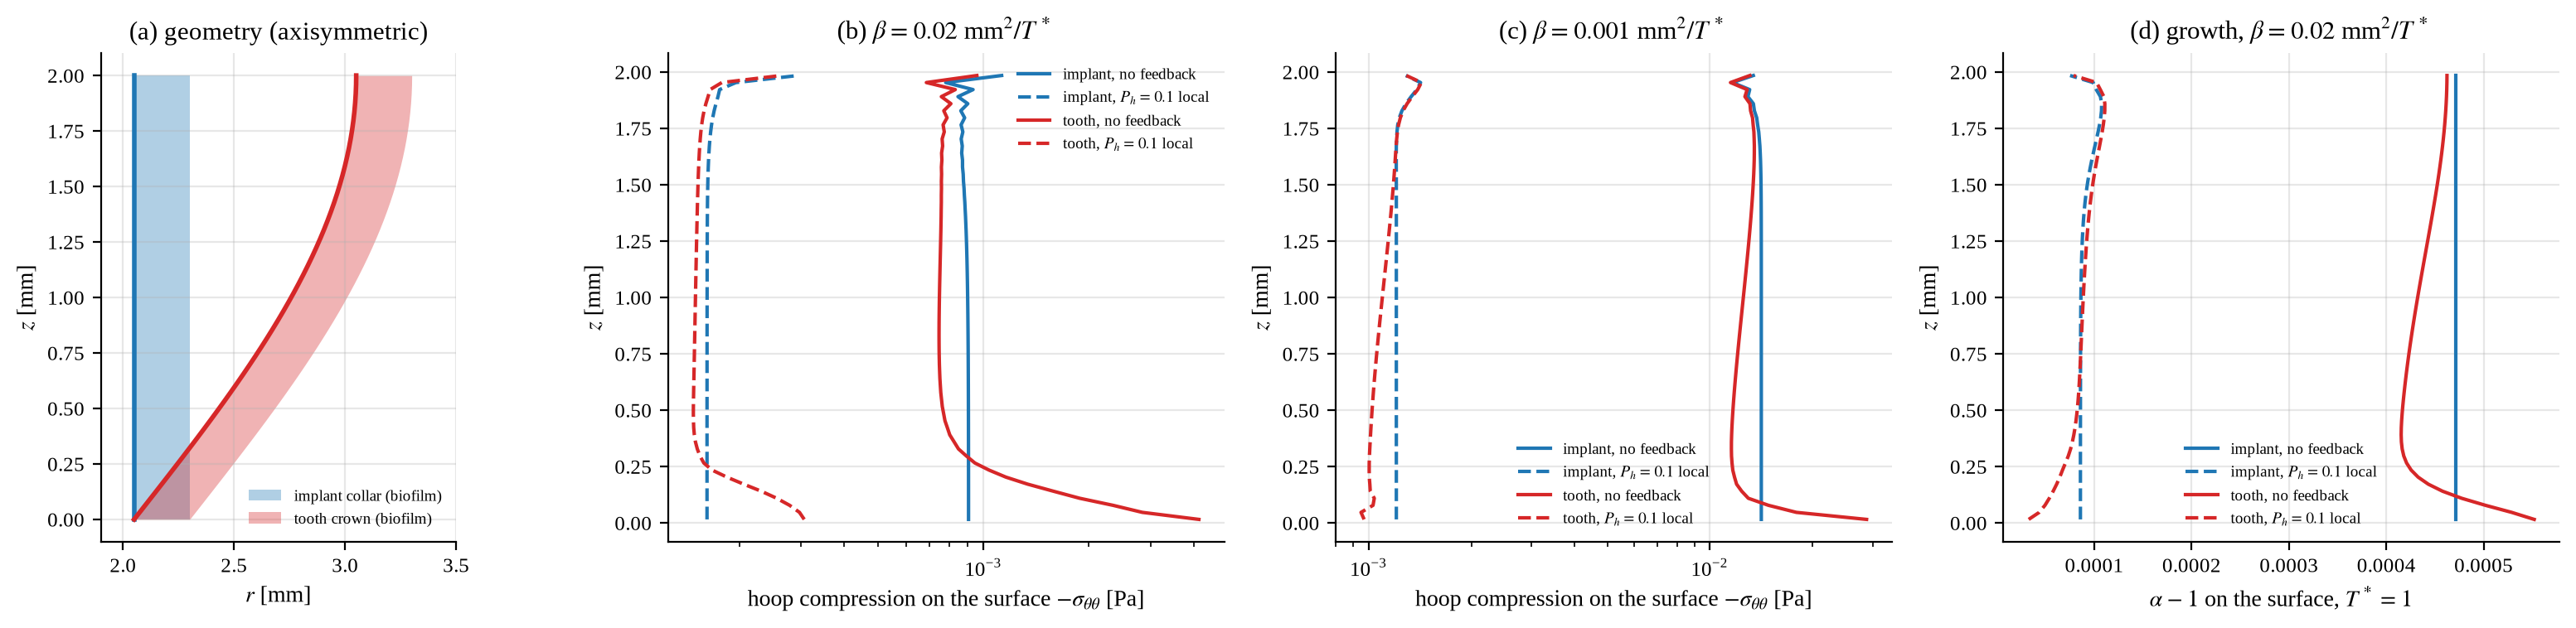
\includegraphics[width=\linewidth]{assets/fig_tooth_homeostatic.png}

\small
\begin{itemize}
  \item 成長の量と帰還の効き方は形でほとんど変わらない（$P_h=0.1$ で 0.80 と 0.31，両方の形で同じ）。
  \item 歯では歯頸線（$z=0$）で周方向応力がインプラントの約 4 倍（$\beta=0.02$）。下面を自由にしても 2 倍残る。
  \item 角の値はメッシュに依存するので，大きさより場所として見る。
\end{itemize}
\end{frame}

% --------------------------------------------------------
\begin{frame}{付録（予備）：栄養と前線の項を入れると}
\centering
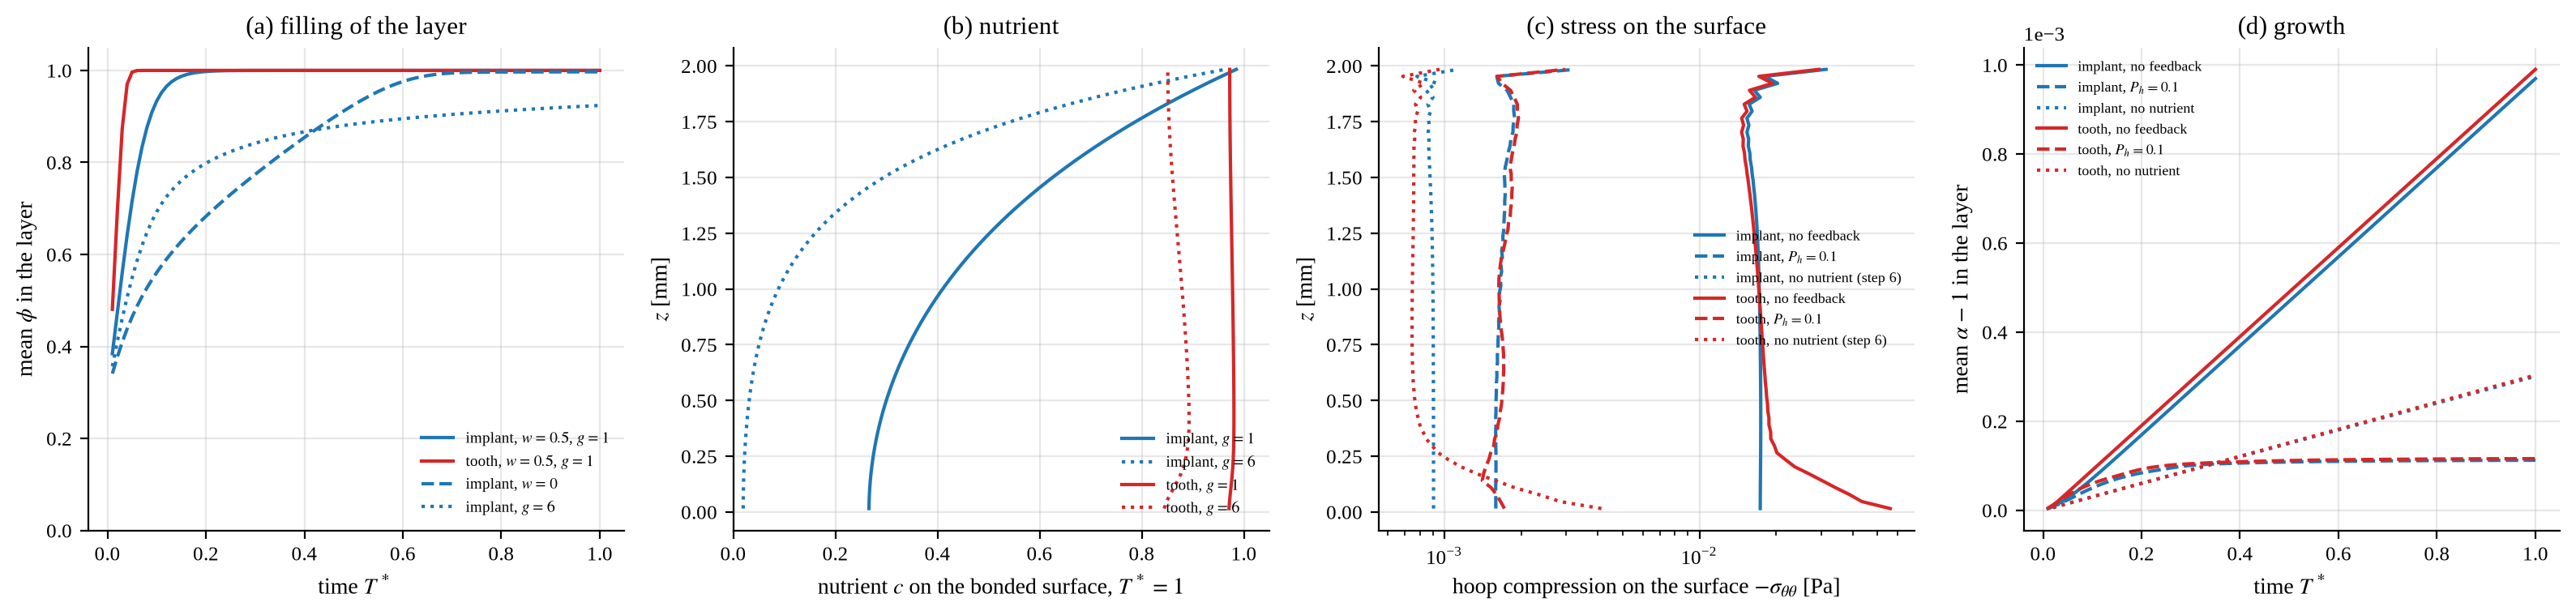
\includegraphics[width=\linewidth]{assets/fig_nutrient_homeostatic.png}

\small
\begin{itemize}
  \item 栄養はインプラントで上面（歯肉縁），歯で外側の面から。$d=1$ mm$^2/T^*$，$g=1/T^*$，$r=10$ mm$/T^*$（Table 2 を 2 mm に換算）。
        前線の項はコロニーの全面で成長する形（$w=0.5$，私の修正）。
  \item 層は $T^*\approx0.1$ までに埋まり，成長は栄養なしの 3 倍，応力は 20〜30 倍。
  \item $P_h=0.1$ の帰還で成長は $T^*\approx0.3$ で止まり（0.12 倍），歯頸線の集中は消える。
\end{itemize}
\end{frame}

% --------------------------------------------------------
\begin{frame}{付録（予備）：帰還があると，応力は境界条件によらない}
\centering
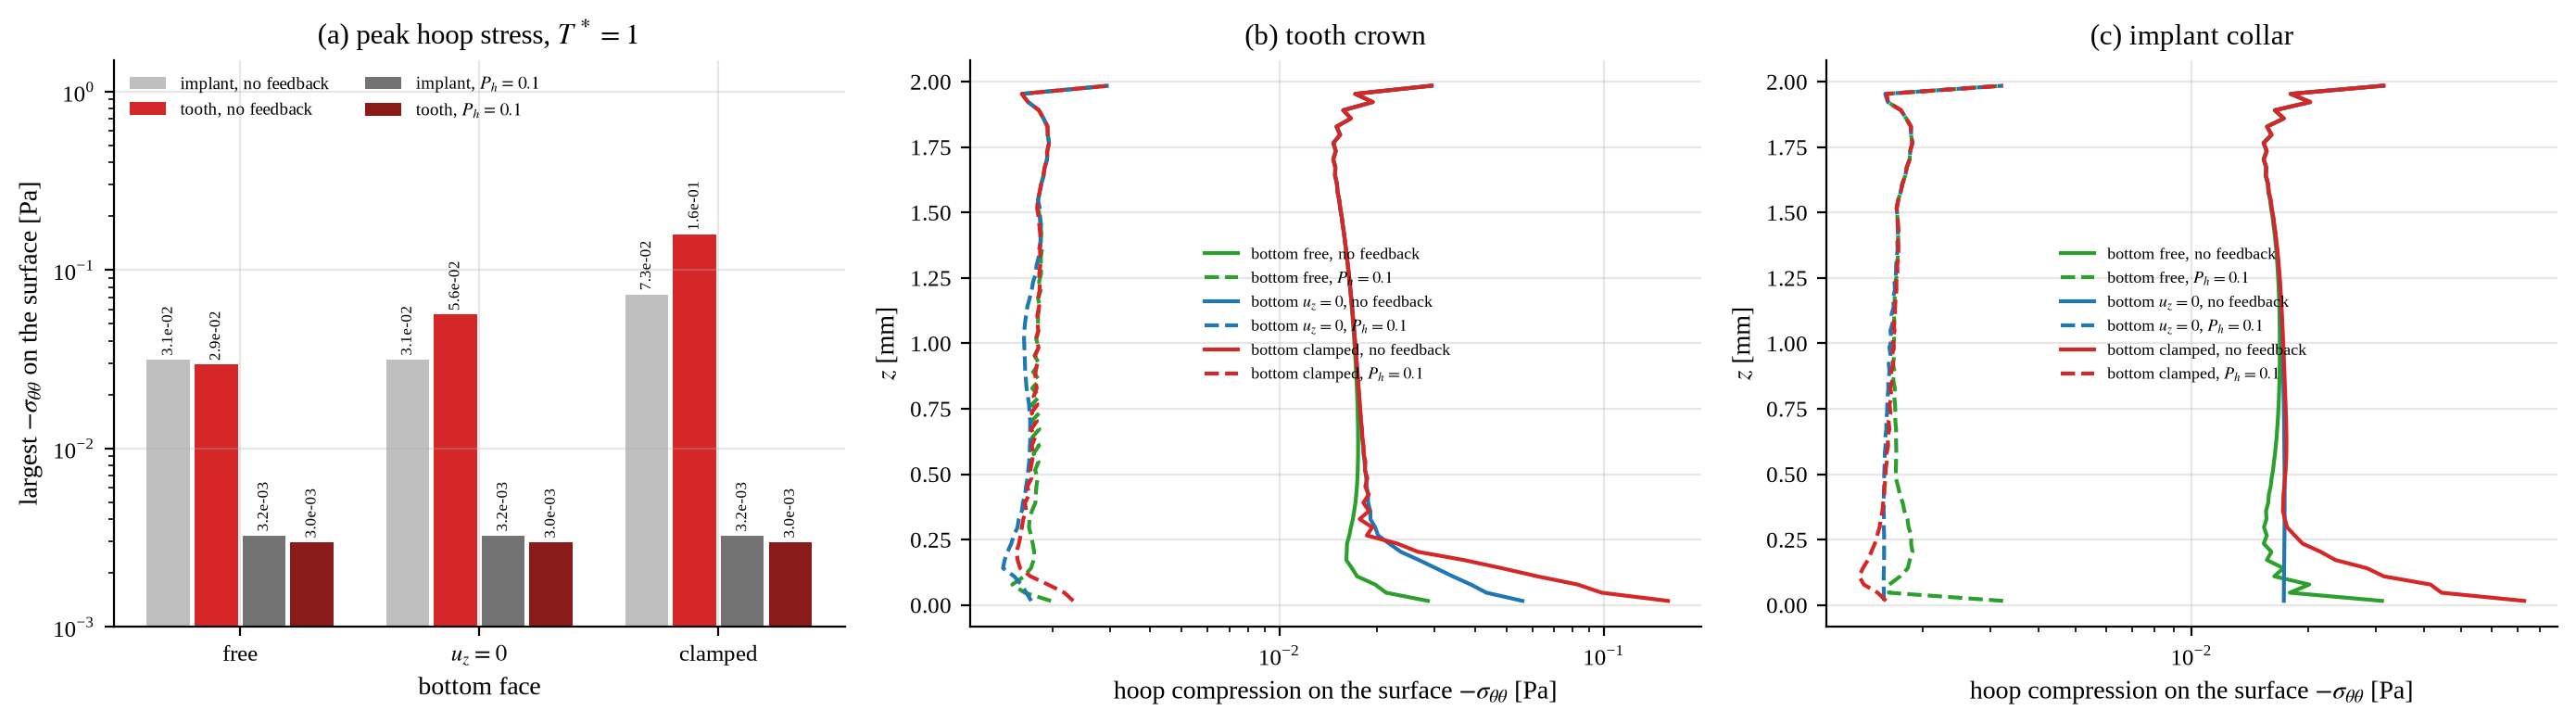
\includegraphics[width=0.98\linewidth]{assets/fig_nutrient_bc.png}

\small
\begin{itemize}
  \item 下面の拘束（自由，$u_z=0$，固定）を変えても，帰還ありの最大の周方向応力は 3.0〜3.2$\times10^{-3}$ Pa。
        帰還なしでは $2.9\times10^{-2}$〜$1.6\times10^{-1}$ Pa と 5 倍の幅がある。
  \item 応力の大きさを決めるのは形や境界ではなく $p_h$。予測は境界の不確かさに強くなるが，$p_h$ を実験から決めることが一番大事になる。
  \item 次：同じ 3 通りを ANSYS／Abaqus の 3 次元で確かめる。
\end{itemize}
\end{frame}

\end{document}
